\subsubsection{Exemple de tableau à 2 dimensions}

Nous allons travailler avec un tableau de type \Tchar, qui implique que chaque élément
n'a besoin que d'un octet en mémoire.

\myparagraph{Exemple de remplissage d'une ligne}
\myindex{\olly}

Remplissons la seconde ligne avec les valeurs 0..3:

\lstinputlisting[caption=Exemple de remplissage d'une ligne,style=customc]{patterns/13_arrays/5_multidimensional/two1_FR.c}

Les trois lignes sont entourées en rouge.
Nous voyons que la seconde ligne a maintenant les valeurs 0, 1, 2 et 3:

\begin{figure}[H]
\centering
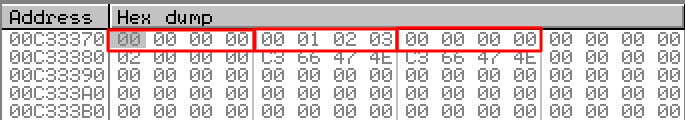
\includegraphics[width=0.6\textwidth]{patterns/13_arrays/5_multidimensional/olly_2D_1.png}
\caption{\olly: le tableau est rempli}
\end{figure}

\myparagraph{Exemple de remplissage d'une colonne}
\myindex{\olly}

Remplissons la troisième colonne avec les valeurs: 0..2:

\lstinputlisting[caption=Exemple de remplissage d'une colonne,style=customc]{patterns/13_arrays/5_multidimensional/two2_FR.c}

Les trois lignes sont entourées en rouge ici.

Nous voyons que dans chaque ligne, à la troisième position, ces valeurs sont écrites:
0, 1 et 2.

\begin{figure}[H]
\centering
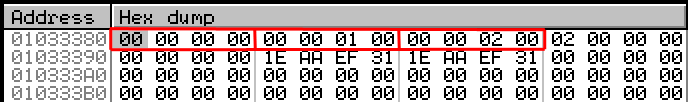
\includegraphics[width=0.6\textwidth]{patterns/13_arrays/5_multidimensional/olly_2D_2.png}
\caption{\olly: le tableau est rempli}
\end{figure}

